\chapter{Serverless design patterns} \label{cha:patterns}

In this chapter we take a look at serverless design patterns. Design patterns describe commonly accepted, reusable solutions to recurring problems \parencite{hohpe2004enterprise}. A design pattern is not a one-size-fits-all solution directly translatable into software code, but rather a formalized best practice that presents a common problem in its context along a general arrangement of elements that solves it \parencite{gamma94designPatterns}. The patterns in this chapter are sourced from scientific literature on serverless computing as well as cloud provider documentation. Literature on object-oriented patterns \parencite{gamma94designPatterns}, SOA patterns \parencite{rotem12soa} and enterprise integration patterns \parencite{hohpe2004enterprise} was also reviewed for applicable practices.

Enterprise integration patterns, as serverless is all about integrations. \textcite{hohpe2004enterprise} present a number of asynchronous messaging architectures in the seminal book on EIP. While predating the whole serverless phenomenon the patterns are still relevant. Hohpe even demonstrated implementing one of his patterns on top of Google's serverless platform \href{http://www.enterpriseintegrationpatterns.com/ramblings/google_cloud_functions.html}{in a blog post}. E.g. patterns like Idempotent Receiver, Dead-letter Channel as well as the 4 more general integration styles of File Transfer, Shared Database, RPC and Messaging. Many patterns implemented internally by FaaS platforms already!

SOA patterns: FaaS functions are self-contained nanoservices these might have some relevance. SOA patterns \parencite{rotem12soa} include Saga, Decoupled Invocation and others. As with EIP, some patterns are already implemented by the FaaS platform.

FaaSification: \textcite{spillner17transformpython} describes an automated approach to transform monolithic Python code into modular FaaS units by partially automated decomposition. Doesn't really seem suitable for the web application migration process covered in this thesis but worth mentioning.

\section{Composition patterns} \label{sec:compositionPatterns}

The following patterns concern serverless function composition: how to compose and orchestrate serverless functions together into more extensive sequences or workflows?

\subsection{Routing Function} \label{subsec:routingFunction}

\textbf{Problem:} How to branch out execution flow based on request payload?

\begin{figure}[h]
  \centering
  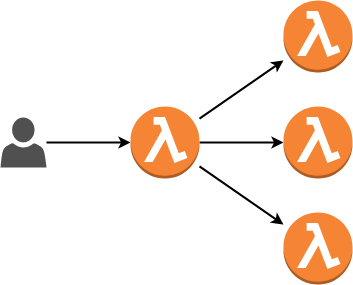
\includegraphics[width=0.4\textwidth]{patterns/routing-function.png}
  \caption{Routing Function}
  \label{fig:patternRoutingFunction}
\end{figure}

\textbf{Solution:} Use a central routing function to receive requests and invoke appropriate functions based on request payload.

This pattern involves instantiating a routing function that contains all the necessary information to route requests to other functions. All function invocations are directed to the routing function, which in turn invokes target functions according to request payload. The routing function finally passes target function return value over to the client.

It's notable that FaaS platforms commonly provide API gateways and other tools for routing, for example the Amazon API Gateway \parencite{awslambda0218}. These tools are however mostly limited to path-based routing, whereas a routing function can be implemented to support more dynamic use cases. Also interestingly, according to an industry survey \parencite{leitner18industrialpractice}, some practicioners opted for the Routing Function pattern over platform API gateway services as they found the latter cumbersome to manage. \textcite{sbarski2017serverless} similarly postulate that the pattern ``can simplify the API Gateway implementation, because you
may not want or need to create a RESTful URI for every type of request''. One advantage of the pattern is that the routing function can be used to supplement request payload with additional context or metadata. A centralized routing function also means that all routing configuration is found in one place, and that public-facing API routes only need to be configured for one function, not all of them \parencite{leitner18industrialpractice}.

The pattern's major disadvantage is double billing, as the routing function essentially has to block and wait until the target function finishes execution. Additionally, as routing is implemented in function code level, information about function control flow gets hidden in implementation rather than being accessible from configuration \parencite{leitner18industrialpractice}.

The Routing Function pattern is related to the OOP Command pattern, which is used to decouple the caller of the operation from the entity that carries out the processing via an intermediary command object \parencite{gamma94designPatterns}. A related enterprise integration pattern is Content-Based Router, which ``examines the message content and routes the message onto a different channel based on data contained in the message'' \parencite{hohpe2004enterprise}. \textcite{hohpe2004enterprise} caution that the router should be made easy to maintain as it can become a point of frequent configuration.

\subsection{Function Chain} \label{subsec:functionChain}

\textbf{Problem:} Task exceeds maximum function execution duration, resulting in a timeout.

\begin{figure}[h]
  \centering
  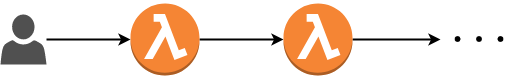
\includegraphics[width=0.5\textwidth]{patterns/function-chain.png}
  \caption{Function Chain}
  \label{fig:patternFunctionChain}
\end{figure}

\textbf{Solution:} Split the task into separate functions that are chained together sequentially.

The Function Chain pattern comprises of an initial function and any number of subsequent functions. The initial function begins computation while keeping track of remaining execution time. In AWS Lambda for example the execution context contains information on how many milliseconds are left before termination \parencite{awslambda0218}. Upon reaching its duration limit, the initial function invokes another function asynchronously, passing along as parameters any state necessary to continue task computation. Since the intermediary invocation is asynchronous (``fire-and-forget''), the initial function can terminate without affecting the next function in chain.

The Function Chain pattern is in effect a workaround over the duration limit that FaaS platforms place on function execution \parencite{leitner18industrialpractice}. The pattern was reported to be used at least occasionally in an industry study by \textcite{leitner18industrialpractice}. Its disadvantages include strong coupling between chained functions, increase in the number of deployment units and the overhead of transferring intermediate execution state and parameters between each chained function. \textcite{leitner18industrialpractice} also note that splitting some types of tasks into multiple functions can be difficult. Finally, as the pattern relies on asynchronous invocation, the last function in chain has to persist computation result into an external storage for the client to access it, which brings in further dependencies.

\subsection{State Machine} \label{subsec:stateMachine}

\textbf{Problem:} How to coordinate complex, stateful procedures with branching steps?

\begin{figure}[h]
  \centering
  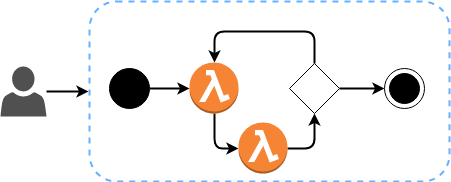
\includegraphics[width=0.6\textwidth]{patterns/state-machine.png}
  \caption{State Machine}
  \label{fig:patternStateMachine}
\end{figure}

\textbf{Solution:} Split a task into a number of discrete functions and coordinate its execution with an orchestration tool.

\textcite{hong18securingviaserverlesspatterns} describe the State Machine pattern as ``building a complex, stateful procedure by coordinating a collection of discrete Lambda functions using a tool such as AWS Step Functions''. These orchestration tools consist of a collection of workflow states and transitions between them, with each state having its associated function and event sources -- essentially a serverless a state machine \parencite{cncf18serverlessWG}. Figure \ref{fig:patternStateMachine} could for example represent a workflow where the first function attempts a database insert, the second function checks whether the operation succeeded, and depending on the result either the operation is retried or execution is finished. The advantage of using provider tooling for workflow execution is that there's no need for external storage as the orchestrator keeps track of workflow state. Downsides on the other hand include extra cost arising from orchestration tooling as well as the overhead of managing workflow descriptions.

\textcite{lopez18orchestration} provide a comparison of three major FaaS orchestration systems: AWS Step Functions, IBM Composer and Azure Durable Functions. The compared systems typically support function chaining, conditional branching, retries and parallel execution, with workflows defined either in a Domain-Specific Language or directly in code. One restriction in Amazon's orchestrator implementation is that a composition cannot be synchronously invoked and is thus not composable in itself: a state machine cannot contain another state machine. AWS Step Functions was also the least programmable among the compared systems, but on the other hand the most mature and performant. Finally, the authors observe that none of the provider-managed orchestration systems are prepared for parallel programming, with considerable overheads in concurrent invocations.

\subsection{Thick Client} \label{subsec:thickClient}

\textbf{Problem:} How to coordinate access to third party cloud services while avoiding extra costs?

\begin{figure}[h]
  \centering
  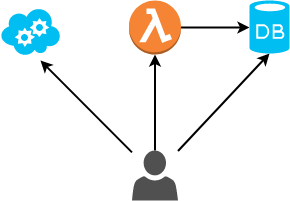
\includegraphics[width=0.5\textwidth]{patterns/thick-client.png}
  \caption{Thick Client}
  \label{fig:patternThickClient}
\end{figure}

\textbf{Solution:} Create thicker, more powerful clients.

Serverless applications, as described in chapter \ref{cha:serverless}, typically rely heavily on third party cloud services (BaaS) interspersed with custom logic in form of serverless functions. In a traditional three-tier web application architecture interaction with these external services would be handled by a server application that sits between the client and the service layers \parencite{robert2016serverlessarchitectures}. Following this model, the client can be limited in functionality whereas the server application plays a larger role. \textcite{sbarski2017serverless} point out that the model of the backend as a gatekeeper between client and services is in conflict with the serverless paradigm. First of all, using FaaS as a middle layer in front of cloud resources directly translates into extra costs: on top of paying for the cloud service call, one has to pay for function invocation and execution for the duration of the network call as well as data transfer between the service and the FaaS provider. Secondly, a middle layer of FaaS results into extra network hops which increases latency and reduces user experience. \textcite{sbarski2017serverless} thus advise against routing everything through a FaaS layer, and advocate building thick clients that communicate directly with cloud services and orchestrate workflows between them.

In addition to the cost benefit, a thicker client has the advantage of improved changeability and separation of concerns, as the single monolithic backend application is replaced by isolated and self-contained components. Doing away with the central arbiter of a server application does come with its trade-offs, including a need for distributed monitoring and further reliance on the security of the cloud services. Importantly not all functionality can or should be moved to the client: security, performance or consistency requirements among others can necessitate a server-side implementation. \parencite{robert2016serverlessarchitectures}.

The Thick Client pattern depends on fine-grained, distributed, request-level authentication in lieu of a gatekeeper server application. This follows naturally from the way serverless functions operate: being stateless and continuously scaling up and down, maintaining a session between the backend and the cloud services is infeasible. Instead of automatically trusting all requests originating from the backend, each cloud service request has to be individually authorized. From a cloud service's point of view, requests originating from a serverless function or directly from the client are both equally untrusted. Hence in serverless architectures, skipping the backend layer is preferable whenever a direct connection between client and services is possible. The Valet Key pattern in section \ref{subsec:valetKey} describes one example of a request-level authentication mechanism. \parencite{adzic2017serverless}

\section{Event patterns} \label{sec:eventPatterns}

Event patterns deal with workflows that are triggered by external events and processed on-demand and asynchronously. FaaS platforms are a good fit for event-driven workflows as they offer integrations to a wide range of event sources as well as non-blocking invocation methods.

\subsection{Event Processor} \label{subsec:Eventprocessing}

\textbf{Problem:} How to execute a piece of business logic on-demand as a result of an event occurrence?

\begin{figure}[h]
  \centering
  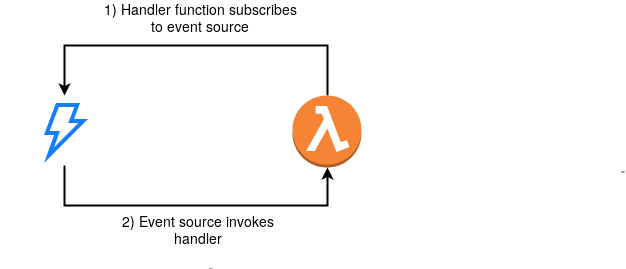
\includegraphics[width=0.45\textwidth]{patterns/event-processor.png}
  \caption{Event Processor}
  \label{fig:patternEventProcessor}
\end{figure}

\textbf{Solution:} Subscribe a serverless function to a cloud event such as a file upload or database change.

The Event Processor pattern consists of one or more serverless functions subscribing to an event from a cloud resource in a way that when the event occurs, the subscribed function is triggered and passed the event context as parameters \parencite{hong18securingviaserverlesspatterns}. Serverless platforms typically offer a number of integration points to events originating from other platform services. For example AWS Lambda functions can be triggered by file uploads, database change events, message queue and notification services, IoT events and many others \parencite{awslambda0218}.

\textcite{baldini17currentTrends} mention thumbnail generation triggered by image upload as an exemplary use case of serverless event processing: a bursty, compute-intensive task triggered on-demand by a cloud event. A traditional approach would be to implement a poller system that regularly checks for new images and generates thumbnails as images are detected. Such a system would require constant operation, and depending on polling interval the design leads to either extra network traffic or potentially long delay between event occurrence and processing. The design is especially wasteful in cases where new images come in infrequently. The serverless event processing pattern, in turn, can bring considerable cost benefit in case of infrequent or irregular workflows as computation is only ran when necessary \parencite{hong18securingviaserverlesspatterns}. Another advantage is scalability, as functions are automatically invoked as per the number of events: a large number of events occurring at once leads to a similarly large number of serverless functions executing in parallel \parencite{hong18securingviaserverlesspatterns}.

One point to keep in mind when implementing serverless event processors is that some cloud event sources operate in at-least-once message delivery semantics: due to the highly distributed and eventually consistent nature of cloud platforms, events are guaranteed to be triggered at least once, not exactly once \parencite{awslambda0218}. This means that the triggered serverless function should in effect act idempotently, meaning that multiple executions with the same context result in the same side effects.

\subsection{Periodic Invocation} \label{subsec:periodicInvocation}

\textbf{Problem:} How to execute a piece of code periodically?

\begin{figure}[h]
  \centering
  
\includegraphics[width=0.4\textwidth]{patterns/periodic-invocation.png}
  \caption{Periodic Invocation}
  \label{fig:patternPeriodicInvocation}
\end{figure}

\textbf{Solution:} Trigger function invocations in regular intervals using a scheduler.

\subsection{Fan-out Events} \label{subsec:FanoutEvents}

Trigger multiple actions from a single event.

\subsection{Fan-out/Fan-in} \label{subsec:FanoutFanin}

Split event handling into parallel functions.

\subsection{Pipes and Filters} \label{subsec:PipesAndFilters}

Handle event stream with a pipeline of small functions.

\section{API patterns} \label{sec:apiPatterns}

Integrating with external systems.

\subsection{API composition} \label{subsec:apiComposition}

Hide multiple API calls under a single function.

\subsection{API aggregation} \label{subsec:apiAggregation}

Hide a sequential multi-step API call under a single function.

\subsection{API async} \label{subsec:apiAsync}

Turn a synchronized API into an async one.

\subsection{Legacy API Proxy/Staged migration} \label{subsec:legacyApi}

Replace a legacy API with a new one step by step, a.k.a. Strangler.

\subsection{Separate FaaS handler from core logic} \label
{subsec:separateHandler}

Separate FaaS handler core logic in code level.

\section{Data management/access patterns} \label{sec:dataManagementPatterns}

Managing state and accessing external resources.

\subsection{Externalized State} \label{subsec:externalizedState}

Store function state in external storage.

\subsection{Valet Key} \label{subsec:valetKey}

Sign tokens for clients to directly access resources.

\subsection{Least privilege IAM role} \label{subsec:LeastprivilegeIAMrole}

Minimize attack surface by reducing function access roles to bare minimum.

\section{Performance and scalability patterns} \label{sec:perfPatterns}

Address FaaS performance issues.

\subsection{Function warming} \label{subsec:FunctionWarming}

Ping a function intermittently to avoid cold starts.

\subsection{Oversized function} \label{subsec:OversizedFunction}

Choose maximum memory allocation to access faster CPU resources and improve cold start latency.

\subsection{Singleton} \label{subsec:Singleton}

Take advantage of function execution context to avoid reinitializing function dependencies.

\section{Resiliency and availability patterns} \label{sec:resiliencyPatterns}

Maximize serverless system resiliency.

\subsection{Bulkhead} \label{subsec:Bulkhead}

Isolate high-latency code into separate functions to avoid resource contention.

\subsection{Flow control/throttling} \label{subsec:Flow control/throttling}

Throttle invocations to avoid DDoSing yourself.

\subsection{Circuit breaker} \label{subsec:Circuit breaker}

Keep track of component availability to avoid cascading failures.

